\documentclass[11pt]{article}

\usepackage{abstract}
\usepackage{algorithm}
\usepackage{algorithmic}
\usepackage{amsmath}
\usepackage{amssymb}
\usepackage{bm}
\usepackage{caption}
\usepackage{CJKutf8}
\usepackage{color}
\usepackage{enumitem}
\usepackage{epsfig}
\usepackage{fancyhdr}
\usepackage{float}
\usepackage{graphics}
\usepackage{graphicx}
\usepackage{geometry}
\usepackage{indentfirst}
\usepackage{lastpage}
\usepackage{listings}
\usepackage{mathdots}
\usepackage{mathpazo}
\usepackage{multirow}
\usepackage{pstricks-add}
\usepackage{pst-blur}
\usepackage{subcaption}
\usepackage{tikz}
\usepackage{wasysym}
\usepackage{xcolor}
\usepackage[BoldFont,SlantFont,CJKsetspaces,CJKchecksingle]{xeCJK}

\allowdisplaybreaks
\DeclareMathOperator*{\argmin}{argmin}
\definecolor{Blue}{rgb}{1.,0.75,0.8}
\definecolor{mygray}{rgb}{0.5,0.5,0.5}
\definecolor{mygreen}{rgb}{0,0.6,0}
\definecolor{mymauve}{rgb}{0.58,0,0.82}
\pagestyle{empty}
\parindent 2em   %段首缩进
\setlength{\parindent}{2em}
\setCJKmainfont[BoldFont=SimHei]{SimSun}
\setCJKmonofont{SimSun}% 设置缺省中文字体
\usetikzlibrary{arrows, automata, calc, shapes}

\newcommand{\HRule}{\rule{\linewidth}{0.5mm}}
\newcommand{\hytt}[1]{\texttt{\hyphenchar\font=\defaulthyphenchar #1}}
\renewcommand{\algorithmicrequire}{\textbf{Input:}}   
\renewcommand{\algorithmicensure}{\textbf{Output:}}  
% \hyphenation{read-Sym-bol re-ad-Space-Tab-New-line str-Tab}

%\footnotesize
\lstset{ %
  backgroundcolor=\color{white},   % choose the background color; you must add \usepackage{color} or \usepackage{xcolor}
  basicstyle=\ttfamily,            % the size of the fonts that are used for the code
  breakatwhitespace=false,         % sets if automatic breaks should only happen at whitespace
  breaklines=true,                 % sets automatic line breaking
  captionpos=b,                    % sets the caption-position to bottom
  commentstyle=\ttfamily\color{mygreen},    
                                   % comment style
  deletekeywords={},               % if you want to delete keywords from the given language
  escapeinside={},                 % if you want to add LaTeX within your code
  extendedchars=true,              % lets you use non-ASCII characters; for 8-bits encodings only, does not work with UTF-8
  frame=single,                    % adds a frame around the code
  keepspaces=true,                 % keeps spaces in text, useful for keeping indentation of code (possibly needs columns=flexible)
  keywordstyle=\color{blue},       % keyword style
  language=C++,                    % the language of the code
  morekeywords={},                 % if you want to add more keywords to the set
  numbers=left,                    % where to put the line-numbers; possible values are (none, left, right)
  numbersep=5pt,                   % how far the line-numbers are from the code
  numberstyle=\tiny\color{mygray}, % the style that is used for the line-numbers
  rulecolor=\color{black},         % if not set, the frame-color may be changed on line-breaks within not-black text (e.g. comments (green here))
  showspaces=false,                % show spaces everywhere adding particular underscores; it overrides 'showstringspaces'
  showstringspaces=false,          % underline spaces within strings only
  showtabs=false,                  % show tabs within strings adding particular underscores
  stepnumber=1,                    % the step between two line-numbers. If it's 1, each line will be numbered
  stringstyle=\color{mymauve},     % string literal style
  tabsize=2,                       % sets default tabsize to 2 spaces
  title=\lstname                   % show the filename of files included with \lstinputlisting; also try caption instead of title
}

\pagestyle{fancy}
\rhead{page \thepage\ of \pageref{LastPage}}
%\chead{}
\lhead{计算机体系结构}
\cfoot{}

\begin{document}

\title{第一章作业}
\author{计算机1202 \quad 张艺瀚\\学号:20123852}
\maketitle

\thispagestyle{fancy}
%\newpage
\normalsize

\section{}

计算顺序(括号内为产生时刻)
\begin{enumerate}
  \item $a_1b_1$(1), $a_2b_2$(2), $a_3b_3$(3), $a_4b_4$(4), $a_5b_5$(5), $a_6b_6$(6)
  \item $a_1b_1 + a_2b_2$(12), $a_3b_3 + a_4b_4$(13), $a_5b_5 + a_6b_6$(14)
  \item $a_1b_1 + a_2b_2 + a_3b_3 + a_4b_4$(17)
  \item $a_1b_1 + a_2b_2 + a_3b_3 + a_4b_4 + a_5b_5 + a_6b_6$(21)
\end{enumerate}

时空图见图\ref{tab: f1}
\begin{figure}[h!]
  \centering
  \begin{tabular}{c|c|c|c|c|c|c|c|c|c|c|c|c|c|c|c|c|c|c|c|c|c|}  % {lccc} 表示各列元素对齐方式,left-l,right-r,center-c
    \cline{2-22}
    5 &   &   & $\times$ & $\times$ & $\times$ & $\times$ & $\times$ & $\times$ &   &   &   & $\times$ & $\times$ & $\times$ &   &   & $\times$ &   &   &   & $\times$ \\ \cline{2-22}
    4 &   & $\times$ & $\times$ & $\times$ & $\times$ & $\times$ & $\times$ &   &   &   &   &   &   &   &   &   &   &   &   &   &   \\ \cline{2-22}
    3 &   &   &   &   &   &   &   &   &   &   & $\times$ & $\times$ & $\times$ &   &   & $\times$ &   &   &   & $\times$ &   \\ \cline{2-22}
    2 &   &   &   &   &   &   &   &   &   & $\times$ & $\times$ & $\times$ &   &   & $\times$ &   &   &   & $\times$ &   &   \\ \cline{2-22}
    1 & $\times$ & $\times$ & $\times$ & $\times$ & $\times$ & $\times$ &   &   & $\times$ & $\times$ & $\times$ &   &   & $\times$ &   &   &   & $\times$ &   &   &   \\ \cline{2-22}
    \multicolumn{1}{r}{} & \multicolumn{1}{c}{1} & \multicolumn{1}{c}{2} & \multicolumn{1}{c}{3} & \multicolumn{1}{c}{4} & \multicolumn{1}{c}{5} & \multicolumn{1}{c}{6} & \multicolumn{1}{c}{7} & \multicolumn{1}{c}{8} & \multicolumn{1}{c}{9} & \multicolumn{1}{c}{10} & \multicolumn{1}{c}{11} & \multicolumn{1}{c}{12} & \multicolumn{1}{c}{13} & \multicolumn{1}{c}{14} & \multicolumn{1}{c}{15} & \multicolumn{1}{c}{16} & \multicolumn{1}{c}{17} & \multicolumn{1}{c}{18} & \multicolumn{1}{c}{19} & \multicolumn{1}{c}{20} & \multicolumn{1}{c}{21} \\ 
  \end{tabular}
  \caption{转移图}
  \label{tab: f1}
\end{figure}

最少21拍

\[ SP = \frac{3\times 6 + 4\times 5}{21} = \frac{38}{21} \]

\[ E = \frac{3\times 6 + 4\times 5}{21\times 5} = \frac{38}{105} \]

\[ TP = \frac{11}{21} \]

\section{}

\subsection{}
进制表{1, 5},进制向量(010001)

转移图见图\ref{fig: f}

\begin{figure}[h!]
  \centering
  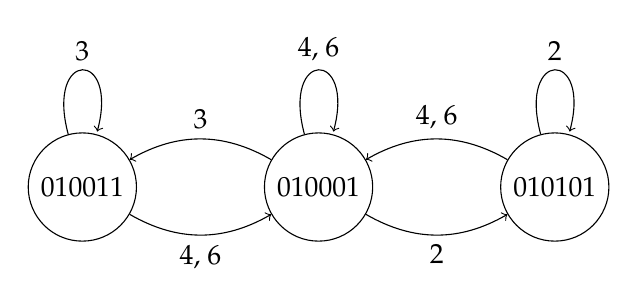
\begin{tikzpicture}[node distance = 3cm, auto]
    \node[state] (q0)                  {010001};
    \node[state] (q1)[left of = q0]    {010011};
    \node[state] (q2)[right of = q0]   {010101};

    \path[->] (q0)    edge[bend right]    node[swap]    {3}     (q1)
              (q1)    edge[bend right]    node[swap]    {4, 6}  (q0)
              (q0)    edge[bend right]    node[swap]    {2}     (q2)
              (q2)    edge[bend right]    node[swap]    {4, 6}  (q0)
              (q0)    edge[loop above]    node          {4, 6}  ()
              (q1)    edge[loop above]    node          {3}     ()
              (q2)    edge[loop above]    node          {2}     ();
  \end{tikzpicture}
  \caption{转移图}
  \label{fig: f}
\end{figure}

\subsection{}
\begin{center}
  \centering
  \begin{tabular}{cc}
  \hline
  调度 & 平均拍数 \\
  \hline
  3, 4 & 3.5 \\
  3, 6 & 4.5 \\
  4 & 4 \\
  6 & 6 \\
  3 & 3 \\
  \textcolor[rgb]{1,0,0}{2} & \textcolor[rgb]{1,0,0}{2} \\
  2, 4 & 3 \\
  2, 6 & 4 \\
  \hline
  \end{tabular}
\end{center}

最佳调度为(2)

\[ TP_{max} = \frac{1}{2} \]

\subsection{}
时空图见图\ref{tab: f2}
\begin{figure}[h!]
  \centering
  \begin{tabular}{c|c|c|c|c|c|c|c|c|c|c|c|c|c|c|c|c|}  % {lccc} 表示各列元素对齐方式,left-l,right-r,center-c
    \cline{2-17}
    $s_4$& &   &   &   & 1 &   & 2 &   & 3 &   & 4 &   & 5 &   & 6 &  \\ \cline{2-17}
    $s_3$& &   &   & 1 &   & 2 &   & 3 &   & 4 &   & 5 &   & 6 &   &  \\ \cline{2-17}
    $s_2$& & 1 & 1 & 2 & 2 & 3 & 3 & 4 & 4 & 5 & 5 & 6 & 6 &   &   &  \\ \cline{2-17}
    $s_1$&1&   & 2 &   & 3 & 1 & 4 & 2 & 5 & 3 & 6 & 4 &   & 5 &   & 6\\ \cline{2-17}
    \multicolumn{1}{r}{} & \multicolumn{1}{c}{1} & \multicolumn{1}{c}{2} & \multicolumn{1}{c}{3} & \multicolumn{1}{c}{4} & \multicolumn{1}{c}{5} & \multicolumn{1}{c}{6} & \multicolumn{1}{c}{7} & \multicolumn{1}{c}{8} & \multicolumn{1}{c}{9} & \multicolumn{1}{c}{10} & \multicolumn{1}{c}{11} & \multicolumn{1}{c}{12} & \multicolumn{1}{c}{13} & \multicolumn{1}{c}{14} & \multicolumn{1}{c}{15} & \multicolumn{1}{c}{16} \\ 
  \end{tabular}
  \caption{转移图}
  \label{tab: f2}
\end{figure}
各作业的完成时间为6,8,10,12,14,16

\[ TP = \frac{6}{16} = \frac{3}{8} \]
\[ SP = \frac{6\times 6}{16} = \frac{9}{4} \]
\[ E = \frac{6\times 6}{16\times 4} = \frac{9}{16} \]

\end{document}
